%<dscrpt>Théorème de Poncelet.</dscrpt>
\noindent \textbf{\large{Définitions et notations}}

\begin{itemize}
\item[\textbullet] Le plan est identifié à $\C$.
\item[\textbullet] On identifie $\mathbb{U} = \{ z\in \C \mid \abs{z} = 1\}$ au cercle de centre $0$ et de rayon $1$ de $\R^{2}$ et on note $\mathbb{D} = \{ z\in \C \mid \abs{z}  < 1\}$.
\item[\textbullet] Pour tout complexe $z$ et tout réel $r>0$, on appelle cercle de centre $z$ et de rayon $r$ l'ensemble $\Gamma_{z, r} = \{ z + re^{it},\ t\in \R \}$. 
\item[\textbullet] Une droite d'équation $ax + by = c$ (avec $a,b,c\in \R$ et $(a, b)\neq (0, 0)$) est identifée à l'ensemble $\{ z\in \C \mid a\operatorname{Re}(z) + b\operatorname{Im}(z) = c\}\subset \C$. 
\item[\textbullet] Pour tout $\alpha \in \R$, on note $\tau_{\alpha}$ la fonction définie par: $\forall t\in \R,\ \tau_{\alpha}(t) = t + \alpha$.
\end{itemize}

\bigskip


{\bf \large Introduction.} Soit $\Gamma$ un cercle contenu dans $\mathbb{D}$ et $z_{0}, z_{1}$ deux points de $\mathbb{U}$ tels que la droite $(z_{0}z_{1})$ soit tangente au cercle $\Gamma$. Notons $z_{2}$ l'unique point de $\mathbb{U}$ distinct de $z_{0}$ tel que $(z_{1}z_{2})$ soit tangente à $\Gamma$. On construit par récurrence une suite $(z_{n})$ en notant, pour tout $n\geq 1$, $z_{n+1}$ l'unique point de $\mathbb{U}$ distinct de $z_{n-1}$ tel que la droite $(z_{n}z_{n+1})$ soit tangente à $\Gamma$. Le but de ce problème est de démontrer le théorème de Poncelet:
\begin{quotation}
soit la suite $(z_{n})_{n\in \N}$ est périodique pour toute valeur de $z_{0}$, soit elle ne l'est pour aucune.  
\end{quotation} 
En d'autres termes, le caractère périodique ou non de la suite $(z_{n})_{n\in \N}$ dépend uniquement de $\Gamma$ et non de $z_{0}$.

\begin{figure}[h!]
  \centering
  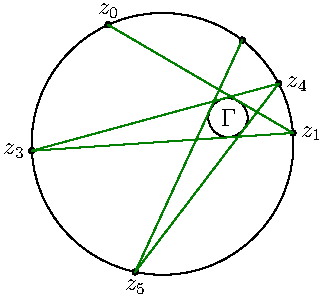
\includegraphics{Eponcelet_1.pdf}
  % Eponcelet_1.pdf: 156x156 px, 72dpi, 5.50x5.50 cm, bb=0 0 156 156
\end{figure}


\subsection*{I. Conjugaison dans $G$}
On note $G$ l'ensemble des fonctions $f\in \Cont^{1}(\R, \R)$ telles que:
\[
 \forall t\in \R,\;  f'(t) > 0 \; \text{ et } \; f(t+2\pi) = f(t) + 2\pi.
\]

\begin{enumerate}
 \item Soit $f\in G$. 
 \begin{enumerate}
  \item Montrer que $\forall (t, n)\in \R \times \Z$, $f(t+2n\pi) = f(t) + 2n\pi$. 
  \item En choisissant judicieusement $n$, montrer que: 
  \[\forall t\in \R,\ f(0) + t - 2\pi \leq f(t) \leq f(2\pi) + t.\]
  \item Montrer que $f$ est une bijection de $\R$ dans $\R$.
 \end{enumerate}
 
 \item Montrer que $\forall (f,g)\in G^2$, $f^{-1}\in G$ et $f\circ g \in G$.
 
 \item Soit $h\in \Cont^{1}(\R, \R_{+}^{*})$ une fonction $2\pi$-périodique à valeurs strictement positives. 
 \begin{enumerate}
   \item Montrer qu'il existe $\varphi \in G$ telle que $\varphi ' = h$ si et seulement si 
   $\displaystyle{\int_{0}^{2\pi}h(t)\ dt = 2\pi}$.
   \item Montrer qu'il existe $\lambda > 0$ et $\varphi \in G$ tels que $\varphi' = \lambda h$.
 \end{enumerate}
 
 \item Deux éléments $f$ et $g$ de $G$ sont dits conjugués dans $G$ s'il existe $\varphi \in G$ telle que $\varphi \circ f \circ \varphi^{-1} = g$.
 \begin{enumerate}
  \item Soit $f\in G$ et $\alpha \in \R$. Supposons $f$ et $\tau_{\alpha}$ conjugués dans $G$. Il existe alors $\varphi \in G$ tel que $\varphi \circ f \circ \varphi^{-1} = \tau_{\alpha}$. Comparer $\varphi'$ et $f' \times (\varphi ' \circ f)$.
  \item Soit $h\in \Cont^{1}(\R, \R_{+}^{*})$ une fonction $2\pi$-périodique à valeurs strictement positives et $f\in G$ telles que $h = f' \times (h\circ f)$.\newline
  Montrer qu'il existe $\alpha \in \R$ tel que $f$ et $\tau_{\alpha}$. 
soient conjugués dans $G$.
 \end{enumerate}


\subsection*{II. L'application de Poncelet}
Soit $z_{0}\in \C$ et $r > 0$ tels que $|z_0| + r <1$. Définissons une fonction à valeurs complexes $z$ et une fonction à valeurs réelles $p$ par:
\[
  \forall t \in \R,\hspace{0.5cm} z(t) = z_0 + re^{it}, \; p(t) = \Re(r + z_0 e^{-it}).
\]

\item Montrer que 
\[
  \forall t \in \R,\hspace{0.5cm} p(t) = \Re\left( z(t)e^{-it}\right), \; |p(t)| < 1, \; p'(t) = \Im \left( z(t)e^{-it} \right).
\]

Définissons des fonctions à valeurs réelles $\varphi_1$ et $\varphi_2$ par:
\[
  \forall t \in \R,\hspace{0.5cm} \varphi_{1}(t) = t + \arccos(p(t)), \; \varphi_{2}(t) = t - \arccos(p(t)).
\]

\item Montrer que $\varphi_{1}, \varphi_{2}\in G$.

\item Posons $f = \varphi_{2}\circ \varphi_{1}^{-1}$. Soit $\theta \in \R$.
\begin{enumerate}
 \item Montrer que: 
 \[ \varphi_{1}^{-1}(\theta) = \frac{\theta + f(\theta)}{2} \quad \text{ et } \quad p(\varphi_{1}^{-1}(\theta)) = \cos\left ( \frac{\theta - f(\theta)}{2}\right ).\]
 \item Montrer que:
 \[ z(\varphi_{1}^{-1}(\theta)) = \frac{e^{if(\theta)} + f'(\theta)e^{i\theta}}{1+f'(\theta)}.\]
 \item En déduire que:
 \[ f'(\theta) = \frac{\abs{e^{if(\theta)} - z(\varphi_{1}^{-1}(\theta))}}{\abs{e^{i\theta} - z(\varphi_{1}^{-1}(\theta))}}.\]
\end{enumerate}

\subsection*{III. Le théorème de Poncelet}
On reprend les notations des parties I et II, en particulier pour les fonctions $z$, $p(t)$ et $f$. On note $x_{0} = \Re(z_0)$ et $y_{0} = \Im(z_0)$ et $\Gamma = \Gamma_{z_{0}, r}$ le cercle de centre $z_0$ et de rayon $r$.

\item Montrer que $\Gamma \subset \mathbb{D}$.

\item Soient $u, q\in \R$ et $\Delta$ la droite d'équation $\cos(u)x + \sin(u)y = q$.
\begin{enumerate}
 \item Montrer que $\Delta \cap \mathbb{U}$ non vide entraine $\abs{q}\leq 1$.
 \item On suppose qu'il existe $\varphi \in \R$ tel que $q = \cos(\varphi)$. Déterminer $\Delta \cap \mathbb{U}$.
\end{enumerate}

\item Notons $D_{t}$ la droite d'équation $\cos(t)x + \sin(t)y = p(t)$. 
\begin{enumerate}
  \item Montrer que $D_{t}\cap \Gamma = \{ z(t)\}$. \newline
On en déduit que $D_t$ est la tangente au cercle $\Gamma$ au point $z(t)$. 

  \item Montrer que $D_{t}\cap \mathbb{U} = \{ e^{i\varphi_{1}(t)}, e^{i\varphi_{2}(t)} \}$. 
\end{enumerate}

\item  Montrer que pour tout $\theta$, les droites $(e^{i\theta}, e^{if(\theta)})$ et $(e^{i\theta}, e^{if^{-1}(\theta)})$ sont les deux tangentes 
à $\Gamma$ passant par $e^{i\theta}$. Que représentent les complexes $z(\varphi_1^{-1}(\theta))$ et $z(\varphi_2^{-1}(\theta))$?
         
\item Montrer qu'il existe $\alpha \in \R$ et $\varphi \in G$ tels que $\varphi \circ f \circ \varphi^{-1} = \tau_{\alpha}$. On pourra faire intervenir une argumentation géométrique.


\item Soit $\theta \in \R$, considérons la suite $(\theta_{n})_{n\in \N}$ définie par $\theta_{0} = \theta$ et  
\[ 
\forall n\in \N,\ \theta_{n+1} = f(\theta_{n}).
\]
  \begin{enumerate}
   \item Pour tout $n\in \N$, exprimer $\theta_{n}$ en fonction de $\tau_{n\alpha}$, $\varphi$ et $\varphi^{-1}$.
   \item Pour tout $n\in \N$, notons $z_{n} = e^{i\theta_{n}}$. \`A quoi correspond géométriquement la suite $(z_{n})_{n\in \N}$?
   \item Sous quelle condition nécessaire et suffisante la suite $(z_{n})_{n\in \N}$ est-elle périodique? Cette condition dépend-elle de $z_{0}$?
  \end{enumerate}


\end{enumerate}
